\section{Lập trình GPU và giao tiếp liên GPU}

\subsection{Tổng quan về GPU và Ứng dụng Deep Learning}
Mặc dù ban đầu được thiết kế cho đồ họa, kiến trúc nhiều lõi tính toán song song dựa trên mô hình SIMD (Single Instruction, Multiple Data) của GPU đã biến nó trở thành GPGPU (General-Purpose computing on GPU). Khả năng này cực kỳ phù hợp với các phép toán ma trận lớn, vốn là hạt nhân của quá trình huấn luyện Deep Learning.

\subsection{Lập trình CUDA: Cấu trúc Host - Device}
Trong hệ sinh thái CUDA do NVIDIA phát triển, phần cứng tính toán được chia làm hai khu vực độc lập: Host (bao gồm CPU và RAM hệ thống) và Device (GPU và VRAM). Hai thành phần này giao tiếp với nhau qua bus PCIe.

\begin{figure}[H]
    \centering
    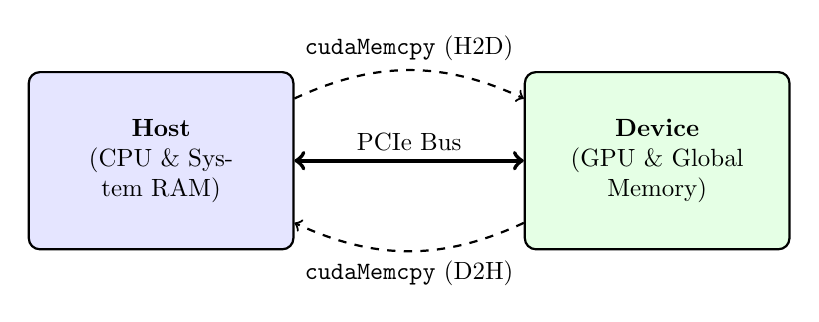
\begin{tikzpicture}[node distance=2cm, auto, thick, scale=0.9, transform shape]
        % Nodes
        \node (cpu) [rectangle, draw, fill=blue!10, text width=3.5cm, text centered, rounded corners, minimum height=2.5cm] {\textbf{Host} \\ (CPU \& System RAM)};
        \node (gpu) [rectangle, draw, fill=green!10, text width=3.5cm, text centered, rounded corners, minimum height=2.5cm, right of=cpu, node distance=7cm] {\textbf{Device} \\ (GPU \& Global Memory)};

        % Edges
        \draw[<->, line width=1.5pt] (cpu) -- node[above] {PCIe Bus} (gpu);
        \draw[->, dashed, bend left=25] (cpu) to node[above] {\texttt{cudaMemcpy} (H2D)} (gpu);
        \draw[->, dashed, bend left=25] (gpu) to node[below] {\texttt{cudaMemcpy} (D2H)} (cpu);
    \end{tikzpicture}
    \caption{Mô hình giao tiếp Host - Device trong kiến trúc CUDA}
    \label{fig:host_device}
\end{figure}

Việc khởi chạy tính toán trên GPU tuân theo quy trình 5 bước cơ bản, được trình bày chi tiết trong Bảng \ref{tab:cuda_steps}.

\begin{table}[H]
\centering
\caption{Quy trình 5 bước cơ bản trong lập trình CUDA}
\label{tab:cuda_steps}
\begin{tabularx}{\textwidth}{|c|l|X|}
\hline
\textbf{Bước} & \textbf{Lệnh CUDA} & \textbf{Mô tả thao tác} \\
\hline
1 & \texttt{cudaMalloc} & Cấp phát bộ nhớ cho Device (Global Memory). \\
2 & \texttt{cudaMemcpy} & Sao chép dữ liệu đầu vào từ Host sang Device. \\
3 & Kernel Launch & Khởi chạy tiến trình tính toán song song trên GPU. \\
4 & \texttt{cudaMemcpy} & Lấy kết quả từ Device về lại Host. \\
5 & \texttt{cudaFree} & Giải phóng bộ nhớ VRAM để tránh rò rỉ. \\
\hline
\end{tabularx}
\end{table}

\subsection{Kiến trúc phần cứng của GPU}
Một vi xử lý GPU bao gồm nhiều Streaming Multiprocessors (SM). Mỗi SM chứa hàng loạt lõi xử lý (Cores/ALUs), bộ nhớ chia sẻ (Shared Memory/L1 Cache). Các luồng thực thi được nhóm lại thành từng cụm 32 luồng gọi là Warp để thi hành chung một lệnh. Về mặt tổ chức logic do CUDA định nghĩa, quá trình tính toán phân cấp từ cao xuống thấp theo cấu trúc: \textbf{Grid $\rightarrow$ Block $\rightarrow$ Thread}. Toàn bộ các luồng đều dùng chung bộ nhớ L2 Cache trung tâm và bộ nhớ toàn cục (Global Memory/VRAM).

\begin{figure}[H]
    \centering
    
\includegraphics[width=0.9\textwidth]{"Figures/Architecture_of_a_CUDA_GPU.JPG"}
    \caption{Kiến trúc phần cứng tiêu biểu của một vi xử lý GPU (CUDA)}
    \label{fig:cuda_arch}
\end{figure}

Cấu trúc tính toán thành 3 tầng từ vĩ mô đến vi mô:
\begin{itemize}
    \item \textbf{Grid}: Cấp độ quản lý cao nhất, chứa toàn bộ các Blocks được sinh ra trong một lần gọi hàm Kernel. Các Blocks trong cùng một Grid hoạt động hoàn toàn độc lập, không thể đồng bộ hóa chéo giữa Block này với Block khác.
    \item \textbf{Block}: Một nhóm chứa nhiều Threads, chúng có thể đồng bộ hóa lịch trình với nhau, và dùng chung một vùng nhớ tốc độ cực cao gọi là Shared Memory.
    \item \textbf{Thread}: Đơn vị thực thi nhỏ nhất và cơ bản nhất. Mỗi luồng sở hữu các thanh ghi (Registers) và vùng Local Memory hoàn toàn độc lập, không luồng nào khác có thể đọc được.
\end{itemize}

\begin{figure}[H]
    \centering
    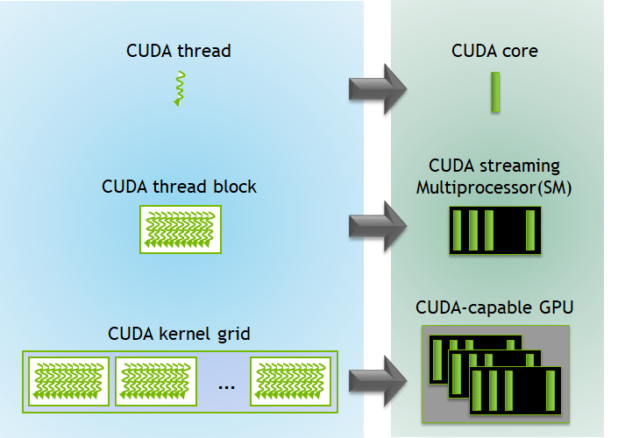
\includegraphics[width=0.7\textwidth]{Figures/kernel-execution-on-gpu-grid-block-thread.png}
    \caption{Cấu trúc phân cấp Grid, Block và Thread trong CUDA}
    \label{fig:grid_block_thread}
\end{figure}

\subsection{Giao tiếp liên GPU: NCCL và NVSHMEM}
Khi bài toán cần sức mạnh của nhiều GPU, giao tiếp giữa chúng quyết định hiệu năng hệ thống.
\begin{itemize}
    \item \textbf{NCCL (NVIDIA Collective Communications Library):} Thư viện tối ưu hóa các phép toán giao tiếp tập thể (như All-Reduce, All-Gather) dành riêng cho nền tảng phần cứng NVIDIA (PCIe, NVLink, InfiniBand). NCCL được tích hợp sâu vào PyTorch DDP để đồng bộ gradient.
    \item \textbf{NVSHMEM:} Dựa trên tiêu chuẩn OpenSHMEM, NVSHMEM sử dụng mô hình lập trình PGAS (Partitioned Global Address Space) và bộ nhớ vùng nhớ đối xứng (symmetric heap). Với giao tiếp truyền-nhận một phía (Put/Get), một GPU có thể ghi dữ liệu thẳng vào VRAM của GPU khác mà không cần sự can thiệp của CPU, đem lại độ trễ cực thấp dù đòi hỏi kiểm soát đồng bộ khắt khe (Barriers, Atomics).
\end{itemize}